\chapter{Main Construction}
\label{chapter:main_construction}

Recall the following question discussed in the introduction.

\begin{question}
    Do there exist circle bundles $E \to M$ over an enlargeable manifold $M$, such that the total space $E$ is non-enlargeable? Moreover, do there exist $2$-dimensional real vector bundles $V \to M$, where $V$ admits a complete metric of uniformly positive scalar curvature?
\end{question}

We begin this chapter with an alternative approach to the one presented in \cite{kumar2025circle} for constructing examples addressing the first part of the question. We subsequently build on this construction to obtain an affirmative answer to the second part of the question.  

\section{Construction of Circle Bundles with \psc}

 In this section we construct examples of circle bundles $E \to M$ over enlargeable manifolds $M$ in all dimensions $\mathrm{dim}(M) \geq 4$, such that $E$ admits a \psc-metric. In particular $E$ is non-enlargeable by Theorem \ref{enl:thm:enl_mnf_do_not_admit_psc}. Let us first describe the strategy behind the construction. The existence of a \psc-metric on $E$ will be established as an application of Theorem \ref{psc:thm:existence_result_totally_non_spin}, restated here for convenience:

\vspace{\baselineskip}
\noindent\textbf{Theorem \ref{psc:thm:existence_result_totally_non_spin}.}\itshape\ 
Let $W^{n+1}$ be an oriented cobordism from $M_0$ to $M_1$, $n \geq 5$. Suppose that $M_1$ is a connected totally non-spin manifold, the inlcusion $M_1 \to W$ induces an isomorphism on $\pi_1$ and that $M_0$ carries a psc-metric. Then $M_1$ also carries a psc-metric. In fact the psc-metric on $M_0$ can be extended to a psc-metric on $W$, which is of product form near the boundary. 
\normalfont
\vspace{\baselineskip}

In order to apply this in our case, we make the following two observations, which hold true for any circle bundle $E \to M$ over a closed orientable manifold $M$. 

\begin{enumerate}[label=(\roman*)]
	\item There exists an oriented nullbordism of $E$, namely the total space of the associated disk bundle $DE \to M$,
	\item \label{constr:eq:circle_bundle_observation2} The inclusion $E \cong \partial DE \to DE$ induces an isomorphism on $\pi_1$ if and only if the fibers of $E$ are contractible, that is the inclusion $S^1 \to E$ is trivial on $\pi_1$.
\end{enumerate}

We have already observed in Example \ref{bundles:ex:associated_bundles_part3} that $DE$ is a nullbordism of $E$. Moreover, the structure group of $DE \to M$ acts on fibers by orientation preserving diffeomorphisms. Thus any orientation on $M$ gives rise to an orientation on $DE$, which is uniquely determined by requiring local trivialisations to be orientation preserving. For \ref{constr:eq:circle_bundle_observation2} note that $DE \to M$ is a homotopy equivalence. Hence the diagram 
\[\begin{tikzcd}[column sep=0cm]
	E && DE \\
	& M
	\arrow[from=1-1, to=1-3]
	\arrow[from=1-1, to=2-2]
	\arrow["\simeq", from=1-3, to=2-2]
\end{tikzcd}\]
shows that $E \to DE$ induces an isomorphism on $\pi_1$ if and only if $E \to M$ does. Then the claim follows follows from the long exact sequence of homotopy groups:
\[\begin{tikzcd}
	{\pi_1(S^1)} & {\pi_1(E)} & {\pi_1(M)} & {\pi_0(S^1)}
	\arrow[from=1-1, to=1-2]
	\arrow[from=1-2, to=1-3]
	\arrow[from=1-3, to=1-4]
\end{tikzcd}\]

With these observations in mind, we have to construct circle bundles $E \to M$ with the following properties.

\begin{enumerate}[label = (\Roman*)]
	\item \label{constr:property1} $M$ is enlargeable, orientable and connected,
	\item \label{constr:property2} $E$ is totally non-spin,
	\item \label{constr:property3} The inclusion $S^1 \to E$ is trivial on $\pi_1$.
\end{enumerate}

We define $M$ as the connected sum of three closed manifolds. Let $N^{2n}$ be any $2n$-dimensional orientable totally non-spin manifold. For example take $N:= \CP^2 \times T^{2n-4}$, which is totally non-spin by Lemma \ref{psc:lem:totally_non_spin_lemma} and Example \ref{bundles:ex:cp2_not_spin}. Then consider
\[
M := \CP^n \# T^{2n} \# N.
\] 
Intuitively the bundle $E \to M$ will now look as follows. It is trivial over the summands $T^{2n}$ and $N$, and is given by the canonical bundle $S^{2n+1} \to \CP^n$ over the $\CP^n$ summand (or rather the restriction of this bundle to $\CP^n - D^{2n} \subseteq M$). Schematically:

\vspace{.3cm}
\begin{figure}[ht]
	\centering
	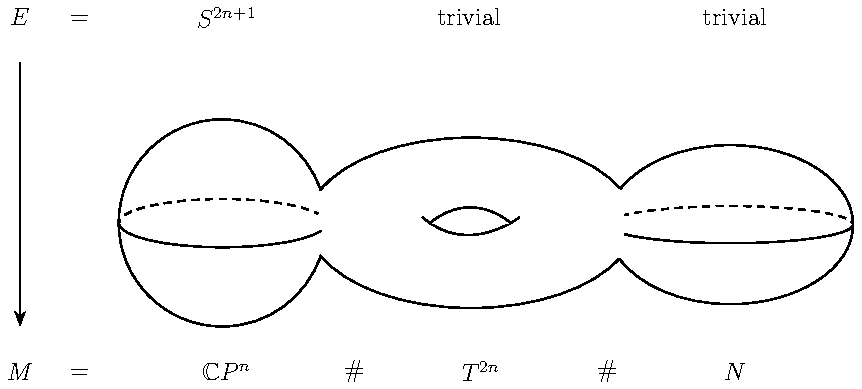
\includegraphics[width=0.95\textwidth]{graphics/main_construction_graphic/main_constr_graphic.pdf}
	\caption{Sketch of the constructed circle bundle}
\end{figure}
\vspace{.1cm}

The presence of the Torus summand then corresponds to property \ref{constr:property1}, the trivial bundle over $N$ to property \ref{constr:property2} and the $S^{2n+1}$ over $\CP^n$ to property \ref{constr:property3}. We will now construct this bundle rigourously and subsequently discuss the proof of properties \ref{constr:property1} - \ref{constr:property3} in more detail. Let $\alpha \in H^2(\CP^n)$ be the generator given boundary the first chern class of the tautological complex line bundle $\tau_1^n \to \CP^n$. Implicitly all homology and cohomology groups in this chapter are taken with $\Z$-coefficients. Consider the isomorphism 
\[
\phi \colon H^2(\CP^n) \oplus H^2(T^{2n}) \oplus H^2(N) \to H^2(M)
\]
and let $c_1 \in H^2(M)$ be the class corresponding to $(\alpha, 0, 0)$ under this isomorphism. By Theorem \ref{bundles:thm:line_bundles_determined_by_chern_class} there exists a unique complex line bundle $L \to M$ with first chern class $c_1(L) = c_1$. Now define $E \to M$ as the $S^1$-principal bundle associated to this line bundle. We claim that $E$ is of the form as described above. To this end we will show that $L \to M$ is trivial over the summands $T^{2n}$ and $N$, and is given by the restriction of $\tau_1^n \to \CP^n$ to $\CP^n - D^{2n} \subseteq M$ over the $\CP^n$ summand. By Example \ref{bundles:ex:associated_bundles} \ref{bundles:ex:associated_bundles_cpn} the associated prinicpal bundle of $\tau_1^n \to \CP^n$ is precisely $S^{2n+1} \to \CP^n$, such that the claim then follows from the naturality of changing the fiber, see Remark \ref{bundles:rem:naturality_change_of_fiber}. To establish the statements made about $L \to M$ let
\[
i \colon N - D^{2n} \to M, \quad i_1 \colon N - D^{2n} \to N
\]
be the inclusions. Then
\[\begin{tikzcd}
	{H^2(M)} & {H^2(N - D^{2n}) } \\
	{H^2(\CP^n) \oplus H^2(T^{2n}) \oplus H^2(N)} & {H^2(N) }
	\arrow["{i^\ast}", from=1-1, to=1-2]
	\arrow["\cong", "\phi"', from=2-1, to=1-1]
	\arrow["{\mathrm{proj.}}", from=2-1, to=2-2]
	\arrow["\cong", "i_1^\ast"', from=2-2, to=1-2]
\end{tikzcd}\]
commutes and therefore $c_1(i^\ast L) =  i*(c_1) = 0$. Again using Theorem \ref{bundles:thm:line_bundles_determined_by_chern_class} we conclude that $i^\ast L$ is trivial. An analogous argument shows triviality of $L$ over the $T^{2n}$ summand. Similiarly, if we denote by 
\[
j \colon \CP^n - D^{2n} \to M, \quad j_1 \colon \CP^{n}-D^{2n} \to \CP^{n}
\]
the inclusions, the diagram
\[\begin{tikzcd}
	{H^2(M)} & {H^2(\CP^n - D^{2n}) } \\
	{H^2(\CP^n) \oplus H^2(T^{2n}) \oplus H^2(N)} & {H^2(\CP^n) }
	\arrow["{j^\ast}", from=1-1, to=1-2]
	\arrow["\cong", "\phi"',from=2-1, to=1-1]
	\arrow["{\mathrm{proj.}}", from=2-1, to=2-2]
	\arrow["\cong", "j_1^\ast"', from=2-2, to=1-2]
\end{tikzcd}\]
commutes and thus $c_1(j^\ast L) = j^\ast(c_1) = j_1^\ast(\alpha) = c_1(j_1^\ast \tau_1^n)$. Hence, applying Theorem \ref{bundles:thm:line_bundles_determined_by_chern_class} once more shows that $j^\ast L$ and $j_1^\ast \tau_1^n$ are isomorphic bundles. This concludes the construction of $E$. Let us now verify properties \ref{constr:property1} - \ref{constr:property3}.



\begin{proof}[\normalfont\textbf{Proof of property \ref{constr:property1}}]
$M$ is connected and orientable, as each summand is. Moreover, since the collapse map $M \to T^{2n}$ has degree $1$ and $T^{2n}$ is enlargeable, it follows from Lemma \ref{enl:lem:constructing_enlargeable_mnf} that $M$ is also enlargeable. 
\end{proof}

\begin{proof}[\normalfont\textbf{Proof of property \ref{constr:property2}}]
Let $i \colon N - D^{2n} \to M$ be the inclusion. We have established above, that
\[
i^\ast E \cong (N- D^{2n}) \times S^1.
\]
From Lemma \ref{psc:lem:totally_non_spin_lemma} \ref{eq:totally_non_spin_lemma1} and \ref{eq:totally_non_spin_lemma3} we conclude that $(N- D^{2n}) \times S^1$ is totally non-spin. Therefore $E$ contains a totally non-spin submanifold of codimension $0$ and so Lemma \ref{psc:lem:totally_non_spin_lemma} \ref{eq:totally_non_spin_lemma2} implies that $E$ is also totally non-spin.
\end{proof}

\begin{proof}[\normalfont\textbf{Proof of property \ref{constr:property3}}]
Intuitively we can contract the fibers over the $S^{2n+1}$ contained in $E$. One way to formalize this is the following. Consider the following commutative diagram, where the rows are taken from the long exact sequences of homotopy groups of the respective fibrations and the vertical maps are induced by inclusions: 
	\[\begin{tikzcd}
	{\pi_2(M)} & {\pi_1(S^1)} & {\pi_1(E)} \\
	{\pi_2(\CP^n - D^{2n})} & {\pi_1(S^1)} & {\pi_1(j^\ast E)} \\
	{\pi_2(\CP^n)} & {\pi_1(S^1)} & {\pi_1(S^{2n+1})}
	\arrow["{\partial_1}", from=1-1, to=1-2]
	\arrow[from=1-2, to=1-3]
	\arrow[from=2-1, to=1-1]
	\arrow["{\partial_2}", from=2-1, to=2-2]
	\arrow["\cong"', from=2-1, to=3-1]
	\arrow["{\mathrm{id}}", from=2-2, to=1-2]
	\arrow[from=2-2, to=2-3]
	\arrow["{\mathrm{id}}"', from=2-2, to=3-2]
	\arrow[from=2-3, to=1-3]
	\arrow[from=2-3, to=3-3]
	\arrow["{\partial_3}", from=3-1, to=3-2]
	\arrow[from=3-2, to=3-3]
\end{tikzcd}\]
The vertical map on the lower left is an isomorphism, because both $\CP^n$ and $\CP^n - D^{2n}$ are simply connected and so by the Hurewicz Theorem
\[\begin{tikzcd}
	{\pi_2(\CP^n-D^{2n})} & {\pi_2(\CP^n)} \\
	{H_2(\CP^n-D^{2n})} & {H_2(\CP^n)}
	\arrow[from=1-1, to=1-2]
	\arrow["\cong", from=1-1, to=2-1]
	\arrow["\cong", from=1-2, to=2-2]
	\arrow[from=2-1, to=2-2]
\end{tikzcd}\]
commutes and the vertical maps are isomorphisms. Since the bottom horizontal map is an isomorphism the same holds for the top horizontal map.
We now claim that $\partial_1$ is surjective. For this it suffices to show surjectivity of $\partial_2$, which in turn is equivalent to surjectivity of $\partial_3$. But this is clear by exactness of the rows and $\pi_1(S^{2n+1}) = 0$. Consequently
\[
\pi_1(S^1) \to \pi_1(E)
\]
is the zero map.
\end{proof}

The above construction now gives examples for circle bundles with positive scalar curvature over enlargeable manifolds $M$ in all even dimensions $\mathrm{dim}(M)\geq 4$. We argue as in \cite{kumar2025circle} to also obtain examples in odd dimensions as follows. Let $E \to M$ be as above and let $\pi \colon M \times S^1 \to M$ be the projection. Then by Example \ref{psc:ex:scalar_curvature_examples} the pullback bundle $\pi^\ast E \cong E \times S^1$ admits a metric of positive scalar curvature. Furthermore the base space $M \times S^1$ is still enlargeable by Lemma \ref{enl:lem:constructing_enlargeable_mnf}. Naturally, the question arises as to what happens in dimensions $\mathrm{dim}(M) \leq 3$. In this case it turns out that no circle bundle $E \to M$ over an enlargeable manifold $M$ admits a metric of positive scalar curvature. This was shown in \cite[Theorem B, Remark 2]{kumar2025circle}.


\section{Necessity of the Enlargeability Assumption in Gromov's Decay Theorem}

In this section we will use the preceeding results to construct examples of $2$-dimensional real vector bundles $V \to M$ over enlargeable manifolds $M$, such that $V$ admits a complete metric of uniformly positive scalar curvature. 

% We have seen above that for non-trivial bundles $V \to M$ condition \ref{intro:eq:gromov_thm_condition_2} need not be satisfied. Nonetheless, this does not yet answer the question of whether this condition is even necessary. In this section we will use the preceeding results to construct counterexamples to the Theorem if one drops condition \ref{intro:eq:gromov_thm_condition_2} entirely. Specifically, we construct vector bundles $V \to M$ over enlargeable manifolds $M$, such that $V$ admits a complete metric of uniformly positive scalar curvature. Then setting $X := V$ and $f := \mathrm{id}$ provides the desired counterexamples.

Let $E \to M$ be a circle bundle as constructed in the previous section. The existence of a \psc-metric on $E$ followed from an application of Theorem \ref{psc:thm:existence_result_totally_non_spin}. However, we did not make use of the full strength of this theorem. Not only do we obtain a \psc-metric on $E$ but also a \psc-metric on the nullbordism $DE$, which is of product form near the boundary. This observation allows for the following construction. Let $g$ be such a \psc-metric on $DE$ and denote the induced metric on $E$ by $g_E$. Choose some collar neighbourhood $\iota \colon E \times [0,1) \to DE$ with respect to which $g$ is in product form, i.e. 
\[
\iota^\ast g = g_E + dt^2.
\]
Moreover, consider the Riemannian manifold $(E \times [1,\infty), g_E + dt^2)$ equipped with the identity as a collar neighbourhood. We can glue this manifold with $(DE, g)$ along the common boundary $E$ to define another Riemannian manifold 
\[
(V^\prime, h) := (E \times [1,\infty) \cup_E DE, (g_E + dt^2) \cup_E g).
\]
We explicitly mention that the smooth structure on $V^\prime$ is defined with respect to the chosen collar neighbourhoods $\iota$ and $\mathrm{id}_{E \times [1,\infty)}$, such that $h$ is indeed smooth. Note that the metrics on both $E \times [1,\infty)$ and $DE$ are complete, therefore $h$ is also complete. Furthermore, $g_E$ is a \psc-metric, hence the scalar curvature of $g_E + dt^2$ is uniformly positive by compactness of $E$ and Example \ref{psc:ex:scalar_curvature_examples} \ref{psc:ex:scalar_curvature_examples4}. The same holds for the scalar curvature of $g$. Consequently, $\scal_h$ is uniformly positive as well. Now consider the map $p_0 \colon E \times [1,\infty) \to M$ defined as the compostion of the projection $E \times [1,\infty) \to E$ and the bundle projection $p \colon E \to M$. Together with the bundle projection $q \colon DE \to M$ we set
\[
\pi := p_0 \cup_E q \colon V^\prime \to M,
\] 
which we will show to be a rank $2$ vector bundle. However, in general we can only expect $\pi$ to be a continous map as the collar neighbourhood $\iota$ contains no information about the bundle structure on $DE$. To resolve this subtlety, we proceed as follows, being quite precise about the details. Choose trivialisations
\[
\phi_\alpha \colon U_\alpha \times S^1 \to p^{-1}(U_\alpha), \;\; \phi_\beta \colon U_\beta \times S^1 \to p^{-1}(U_\beta)
\]
of $E \to M$ with smooth transition function $\tau_{\alpha\beta} \colon U_\alpha \cap U_\beta \to S^1$. By definition there are then trivialisations
\[
\psi_\alpha \colon U_\alpha \times D^2 \to q^{-1}(U_\alpha), \;\; \psi_\beta \colon U_\beta \times D^2 \to q^{-1}(U_\beta)
\]
of $DE \to M$ with the same transition function $\tau_{\alpha\beta}$. Let $B \subseteq \R^2$ be the open ball of radius $1$ and consider the diffeomorphism
\[
\mu \colon \R^2 - B \to S^1 \times [1,\infty), \; w \mapsto \left( \frac{w}{\abs{w}}, \abs{w} \right),
\]
which is equivariant under the canonical $S^1$-actions. Then we can define a trivialisation
\[
\theta_\alpha \colon U_\alpha \times (\R^2 - B) \xrightarrow{\mathrm{id} \times \mu} U_\alpha \times S^1 \times [1,\infty) \xrightarrow{\phi_\alpha \times \mathrm{id}} p^{-1}(U_\alpha) \times  [1,\infty) = p_0^{-1}(U_\alpha)
\]
of $E \times [1,\infty)$ and similiarly $\theta_\beta \colon U_\beta \times (\R^2 - B) \to p_0^{-1}(U_\beta)$. By construction, the transition function of these trivialisations is again $\tau_{\alpha\beta}$. The maps $\theta_\alpha$ and $\psi_\alpha$ now glue together to a \textit{homeomorphism} 
\[
\xi_\alpha \colon U_\alpha \times \R^2 = (U_\alpha \times (\R^2 - B)) \cup (U_\alpha \times D^2)\xrightarrow{\theta_\alpha \cup \psi_\alpha} p_0^{-1}(U_\beta) \cup q^{-1}(U_\beta) = \pi^{-1}(U_\alpha).
\] 
Likewise we obtain a homeomorphism $\xi_\beta \colon  U_\beta \times \R^2 \to \pi^{-1}(U_\beta)$. From the discussion about the transition functions we conclude 
\[
(\xi_\beta^{-1} \circ \xi_\alpha)(x,w) = (x, \tau_{\alpha\beta}(x) \cdot w).
\]
Observe that this map is smooth. Therefore, the collection of maps constructed in the same manner as $\xi_\alpha$ define a smooth structure on $V^\prime$. This structure may not agree with the one previously defined with respect to the collar neighbourhoods, so for clarity let us refer to the topological manifold $V^\prime$ equipped with this new smooth structure as $V$. Then the map $\pi \colon V \to M$ is clearly smooth and carries the structure of a \textit{smooth} rank $2$ vector bundle. To now obtain a complete metric on $V$ with uniformly positive scalar curvature we recall the following. The smooth structure on $V^\prime$ (defined via the collar neighbourhoods) is up to diffeomorphism the unique smooth structure on the topological manifold $V^\prime$, such that the topological embeddings 
\[
E \times [1,\infty) \to V^\prime, \; \; DE \to V^\prime
\]
are smooth embeddings [hcbord, Theorem 1.4]. Note that the inclusion $E \times [1,\infty) \to V$ is locally given by the inlcusion
\[
U_\alpha \times (\R^2 - B) \to U_\alpha \times \R^2 
\]
with respect to the smooth trivialisations $\theta_\alpha$ and $\xi_\alpha$. Similiarly the inclusion $DE \to V$ is locally given by the inlcusion 
\[
U_\alpha \times D^2 \to U_\alpha \times \R^2 
\]
with respect to $\psi_\alpha$ and $\xi_\alpha$. Hence we conclude from the uniqueness statement above that there exists a diffeomorphism $f \colon V \to V^\prime$. Then the metric $f^\ast h$ on $V$ is complete and of uniformly positive scalar curvature.

